\chapter{Annexes}

\section*{Chronologie des éditions}
\addcontentsline{toc}{section}{Chronologie des éditions}

\begin{figure}[ht]
    \centering
    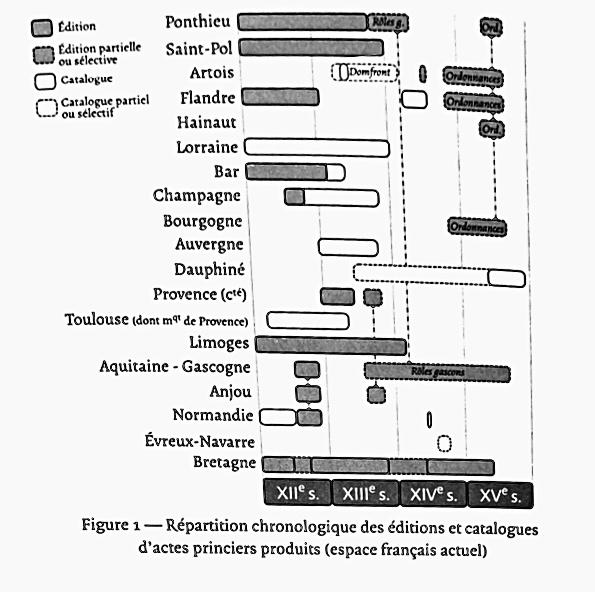
\includegraphics[scale=0.6]{img/repartition_chronologique_editions.jpeg}
    \caption*{Canteaut, Olivier, Moufflet, Jean-François, « Les éditions d’actes princiers (\textsc{XII}\up{e} - \textsc{XV}\up{e} siècle) : bilan à l’ère du numérique », in : Olivier Guyotjeannin et Olivier Mattéoni (éd.), Jean de Berry et l’écrit : Les pratiques documentaires d’un fils de roi de France, Éditions de la Sorbonne, École Nationale des Chartes, Paris, 2019 (Histoire ancienne et médiévale, 159).}
    \label{fig:chrono_ed}
\end{figure}

\section*{Généalogie de la famille ducale de Bourbon}
\addcontentsline{toc}{section}{Généalogie de la famille ducale de Bourbon}

\begin{figure}[H]
\centering
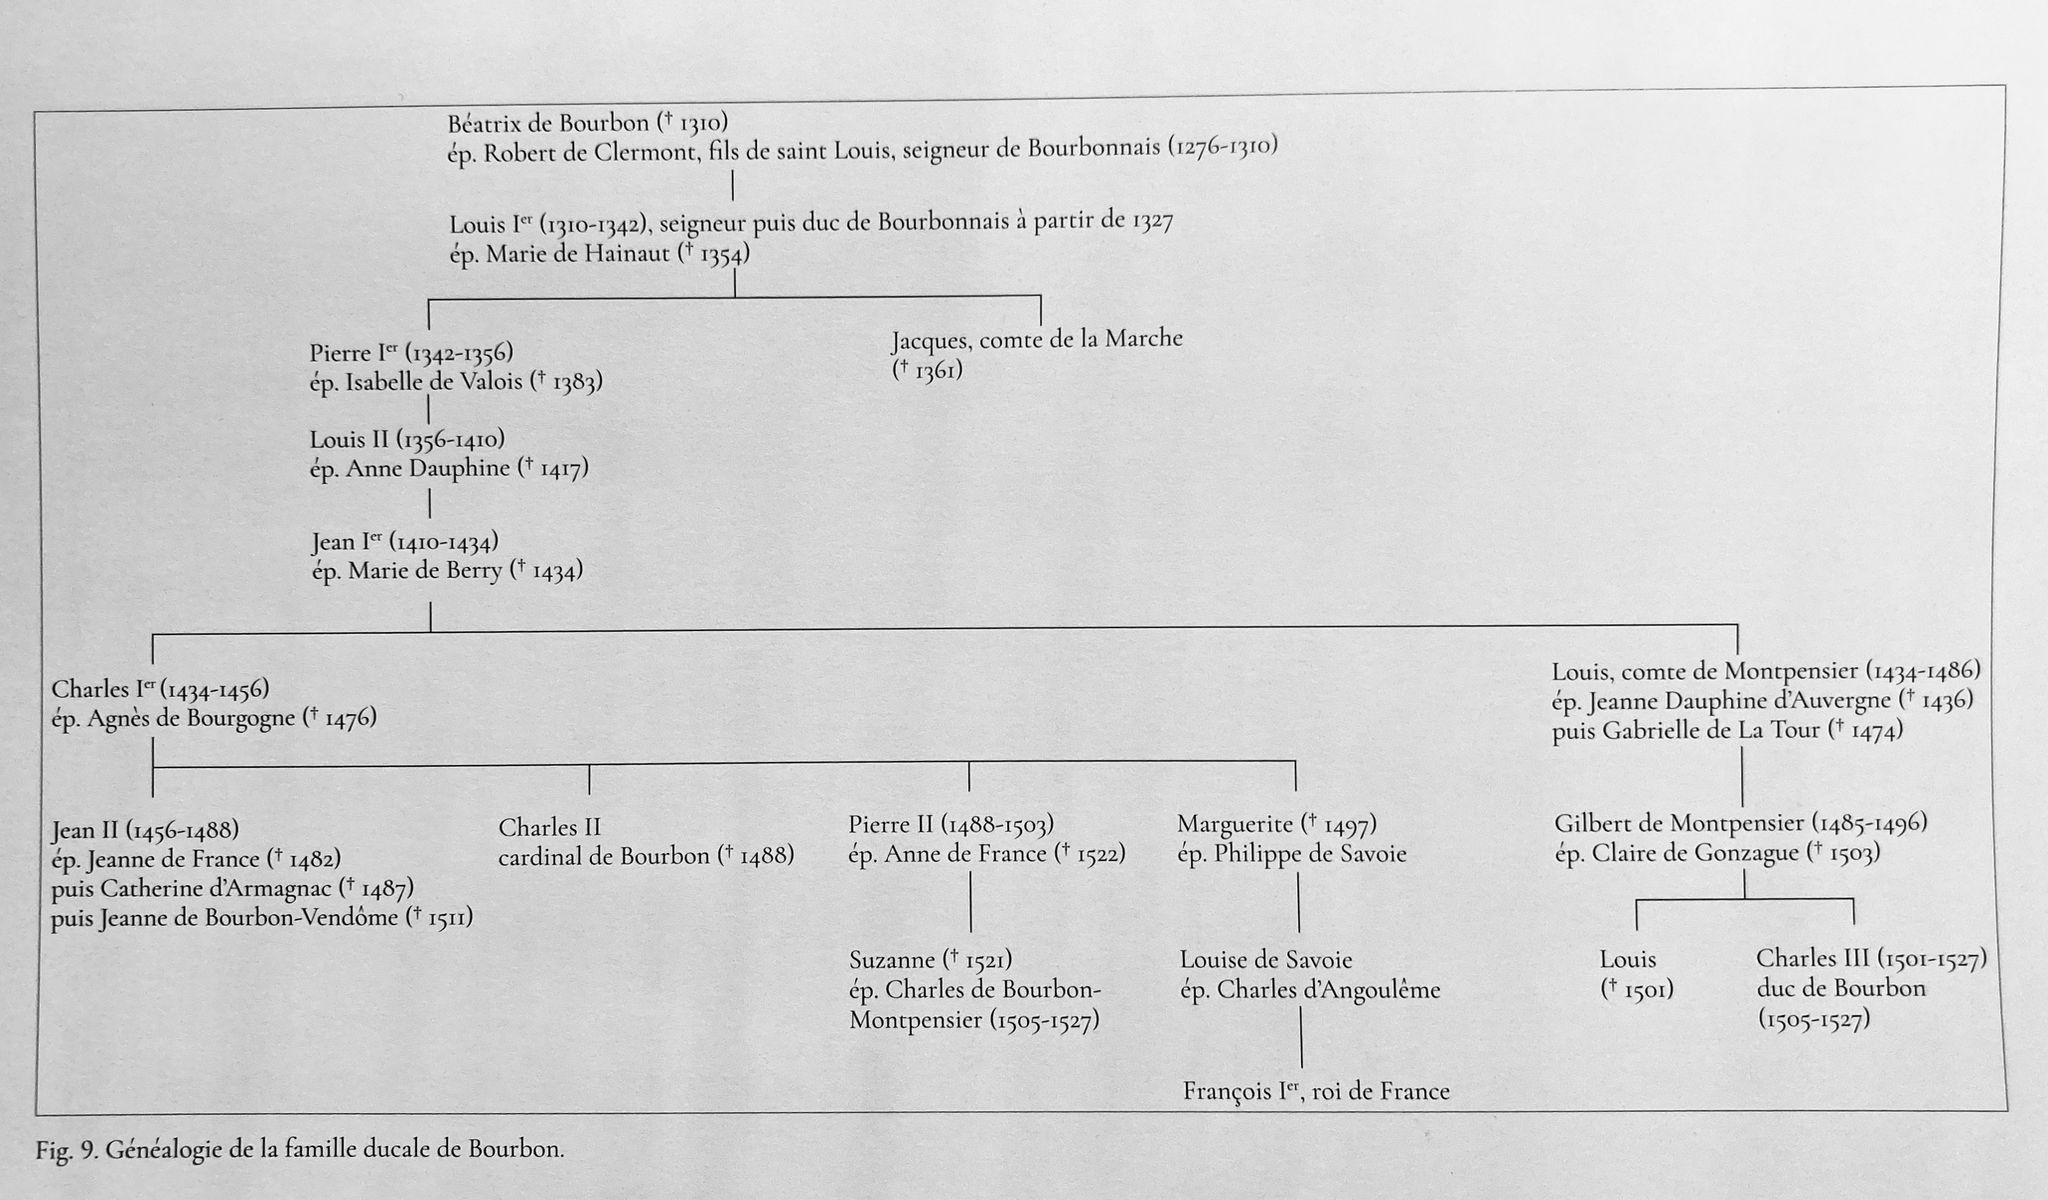
\includegraphics[scale =0.22]{img/genealogie.jpeg}
\caption*{Généalogie de la famille ducale de Bourbon, in \cite{matteoniBourbonsLeurBibliotheque2022}.}
\label{genealogie}
\end{figure}
\newpage 

\section*{Initiales fleurdelisées}
\addcontentsline{toc}{section}{Initiales fleurdelisées}

 \begin{figure}[H]
\centering
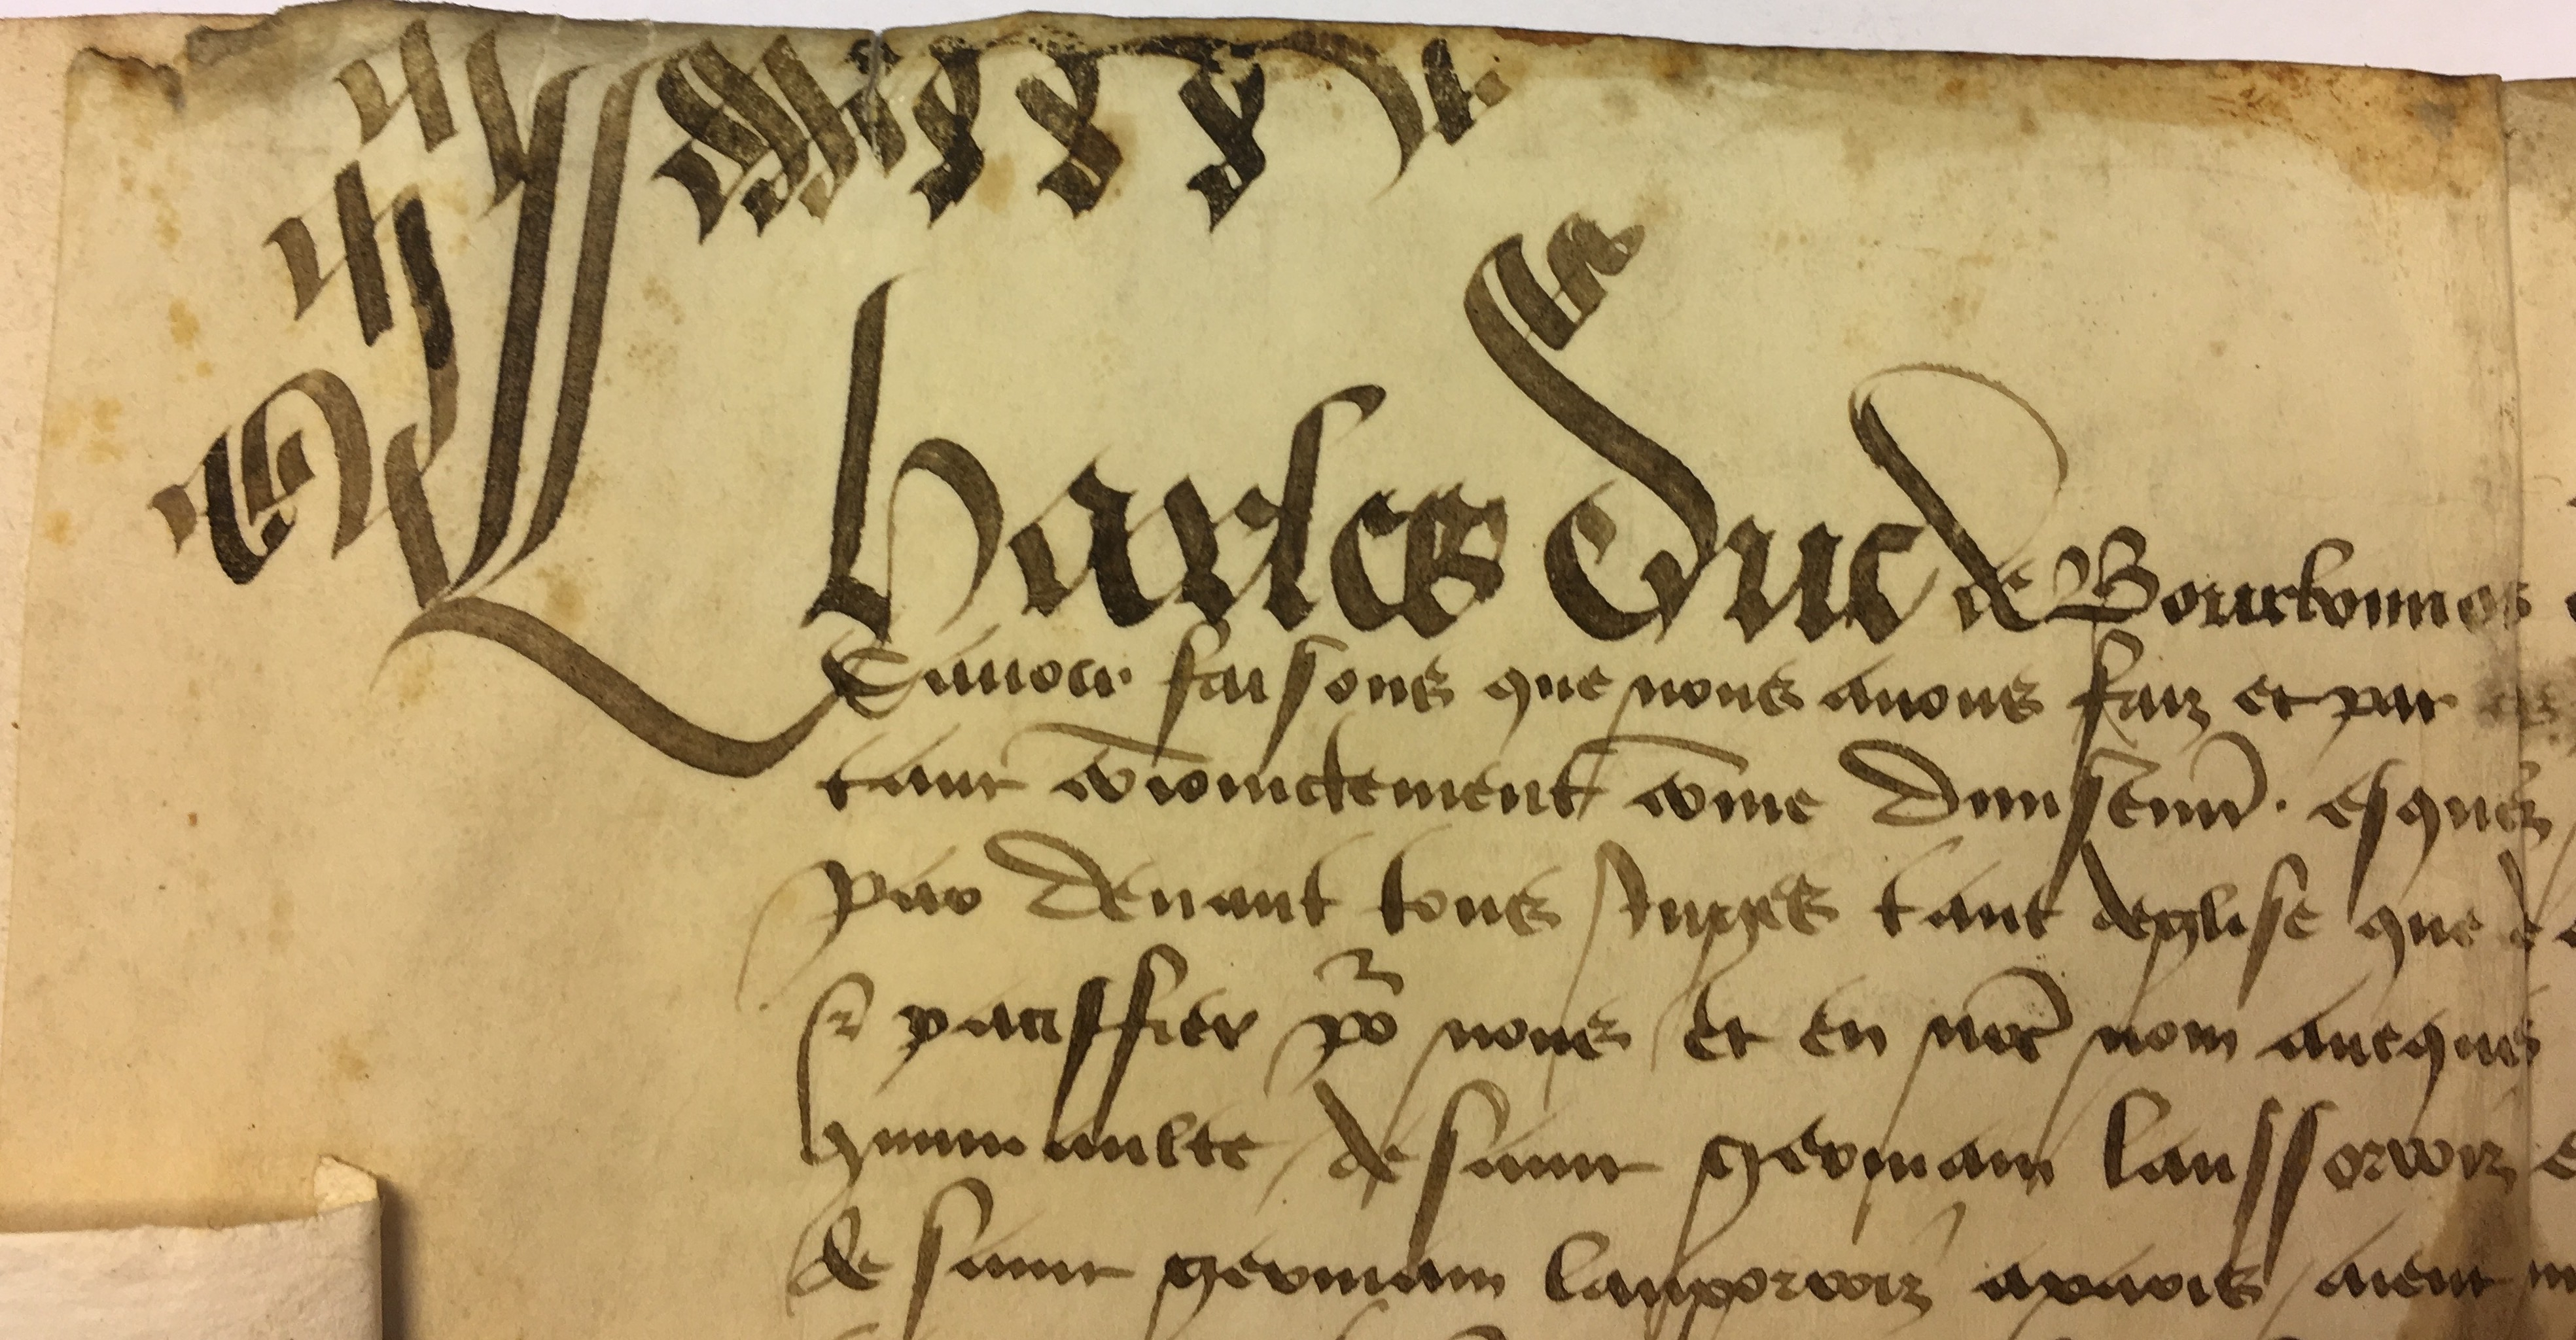
\includegraphics[scale =0.09]{img/fleurlys1.jpg}
\caption*{AN, P 13631, c. 11511 (18 décembre 1448).}
\label{fl1}
\end{figure}

\begin{figure}[H]
\centering
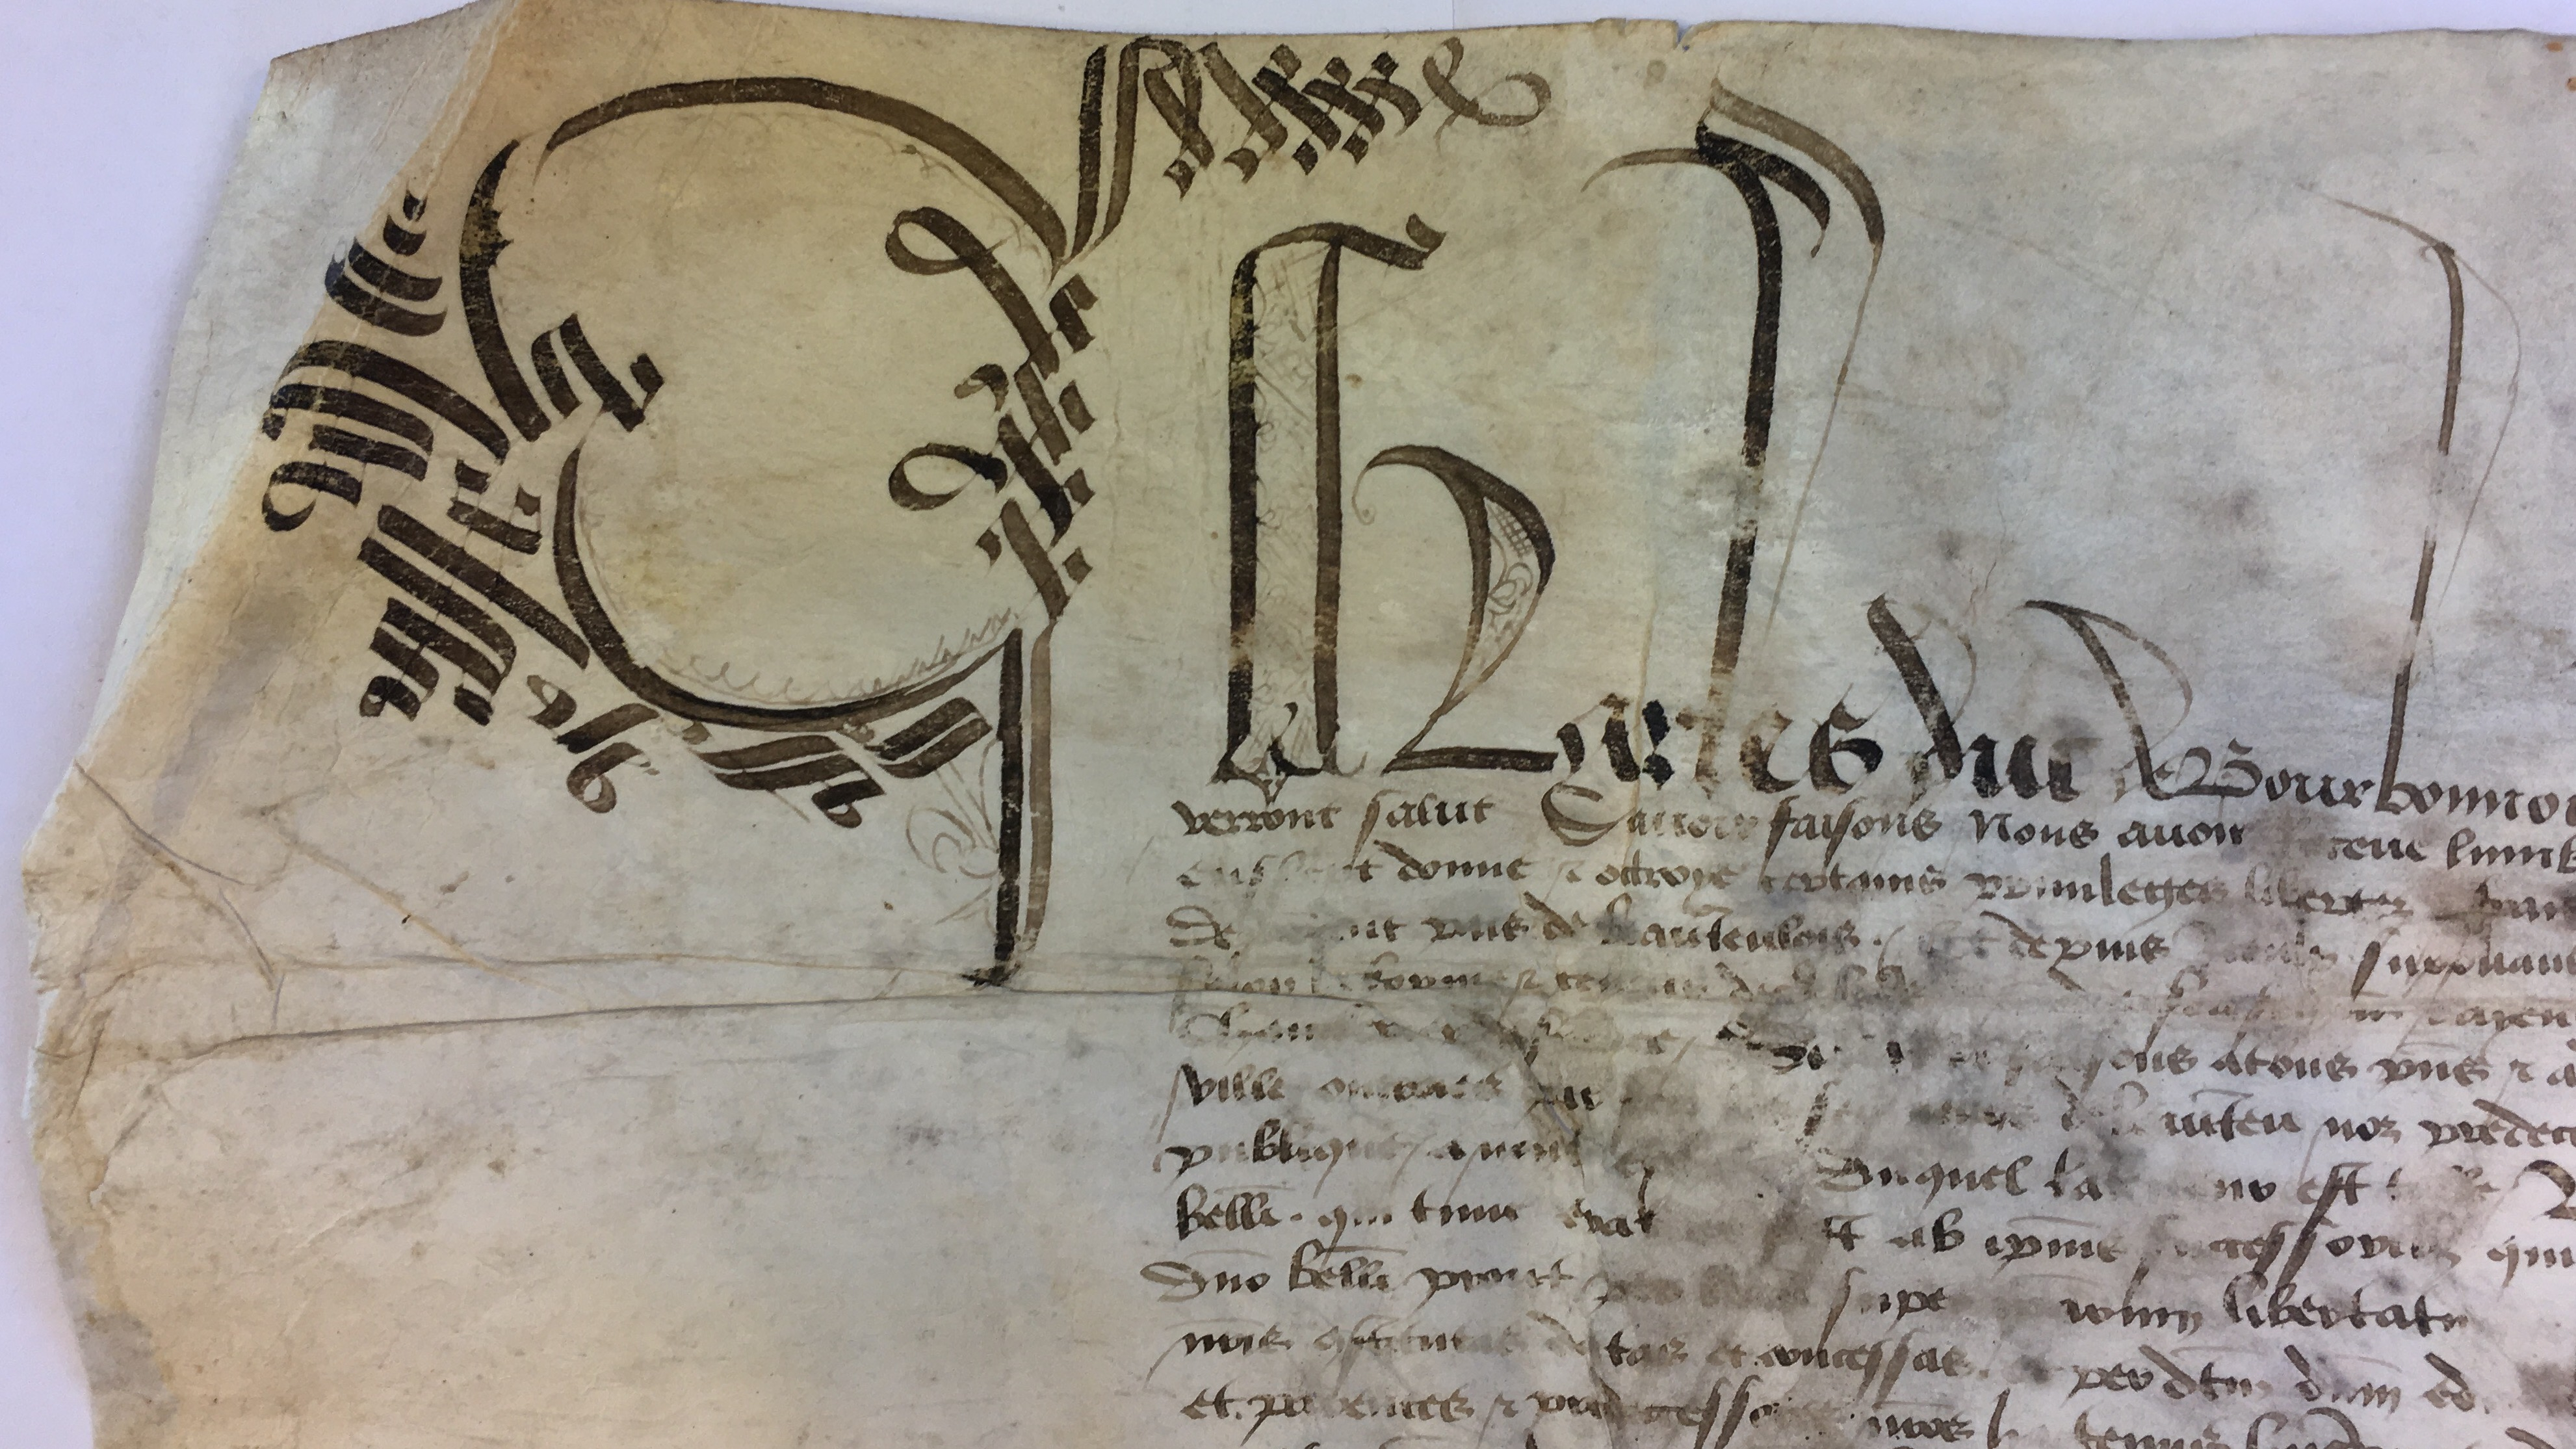
\includegraphics[scale =0.09]{img/fleurlys2.jpg}
\caption*{AN, P 13682, c. 1628 (19 février 1447).}
\label{fl2}
\end{figure}
\newpage 

 \section*{Liste des regex utilisées}
 \addcontentsline{toc}{section}{Liste des regex utilisées}
 
\begin{center}
\begin{longtable}{|l|l|l|}

\hline 
\multicolumn{1}{|c|}{\textbf{Action}} & \multicolumn{1}{c|}{\textbf{Regex}} & \multicolumn{1}{c|}{\textbf{Remplacement}} \\ \hline 
\endfirsthead

\multicolumn{3}{c}%
{{\bfseries \tablename\ \thetable{} -- Liste des regex utilisées}} \\
\hline \multicolumn{1}{|c|}{\textbf{Action}} & \multicolumn{1}{c|}{\textbf{Regex}} & \multicolumn{1}{c|}{\textbf{Remplacement}} \\ \hline 
\endhead

\hline \multicolumn{3}{|r|}{{}} \\ \hline
\endfoot

\hline \hline
\endlastfoot

Retrait des doubles espaces & \textbackslash s\{2\} &  \\
Retrait des sauts de lignes & \textbackslash n &  \\ 
Retrait des sauts de pages & \textbackslash r &  \\
Retrait des mentions \og Sur &  &  \\
le repli \fg (en blanc) & $\hat{~}\backslash$(Sur le repli\textbackslash) ([$\hat{~}$Par].+) & \textbackslash \$1 \\
  &  &  \\
Stylage et indentation des &  &  \\ notes paléographiques &  — ([b-z]\textbackslash .) & \textbackslash n\$1 \\ 
Suppression des astérisques & (\textbackslash *)+ &  \\
  &  &  \\
Stylage des dates & ($\hat{~}[\backslash[\backslash]\backslash d\backslash-]+($ $\backslash(n\backslash. st\backslash.\backslash))?,.+)$ &  \\  & $\hat{~}$(Avant )?\textbackslash d\{4\}.+ &  \\  &  $\hat{~}(14..+)|\hat{~}\backslash $ [(14.+|Avant.+|Après.+|Entre.+) &  \\  &  $\hat{~}$(14..+)|$\hat{~}\backslash $  [(.+) &  \\
Stylage des analyses & $\hat{~}$?Louis,? duc de Bourbonnais,?.+ &  \\
  & Louis,? duc de Bourbonnais, comte de .+ &  \\ 
  & $\hat{~}$Charles de Bourbon, comte de Clermont.+ &  \\ 
  & $\hat{~}$Quittance de Charles.+ &  \\
  & $\hat{~}$Lettre close.+ &  \\
  & $\hat{~}$Marie de Berry, duchesse de Bourbonnais.+ &  \\
  & $\hat{~}$Lettre de Charles.+ &  \\
  & $\hat{~}$Charles, duc de Bourbonnais.+ &  \\
  & $\hat{~}$Ordonnance de Charles.+  &  \\
  & $\hat{~}\backslash$t[A-Z][a-z].+ &  \\
  & $\hat{~}$Anne Dauphine, duchesse de Bourbonnais.+ & \\
Stylage du tableau de la &  &  \\ 
tradition & $\hat{~}A\backslash.$ $.+|\hat{~}B\backslash.$ $.+$ &  \\
Stylage des mentions & $\hat{~}$Mention :.+ &  \\
  & $\hat{~}$Analyse :.+ &  \\
  & $\hat{~}$Indique :.+ &  \\
Stylage du titre des actes & $\hat{~}\backslash$(deperditum$\backslash$)|$\hat{~}$texte établi.+ & \\
Stylage des mentions hors & (\textbackslash(Sur.+) & \textbackslash n\$1 \\ 
teneurs & \textbackslash(Sur.+|\textbackslash(Sous.+|\textbackslash(A g.+ &  \\
  & (Par madame la duchesse,) &  \\
Stylage des signataires & $\hat{~}\backslash$(Signé :\textbackslash).+ &  \\
  
\end{longtable}
\end{center}

\section*{Actes inédits}
\addcontentsline{toc}{section}{Actes inédits}

\begin{figure}[ht]
\centering
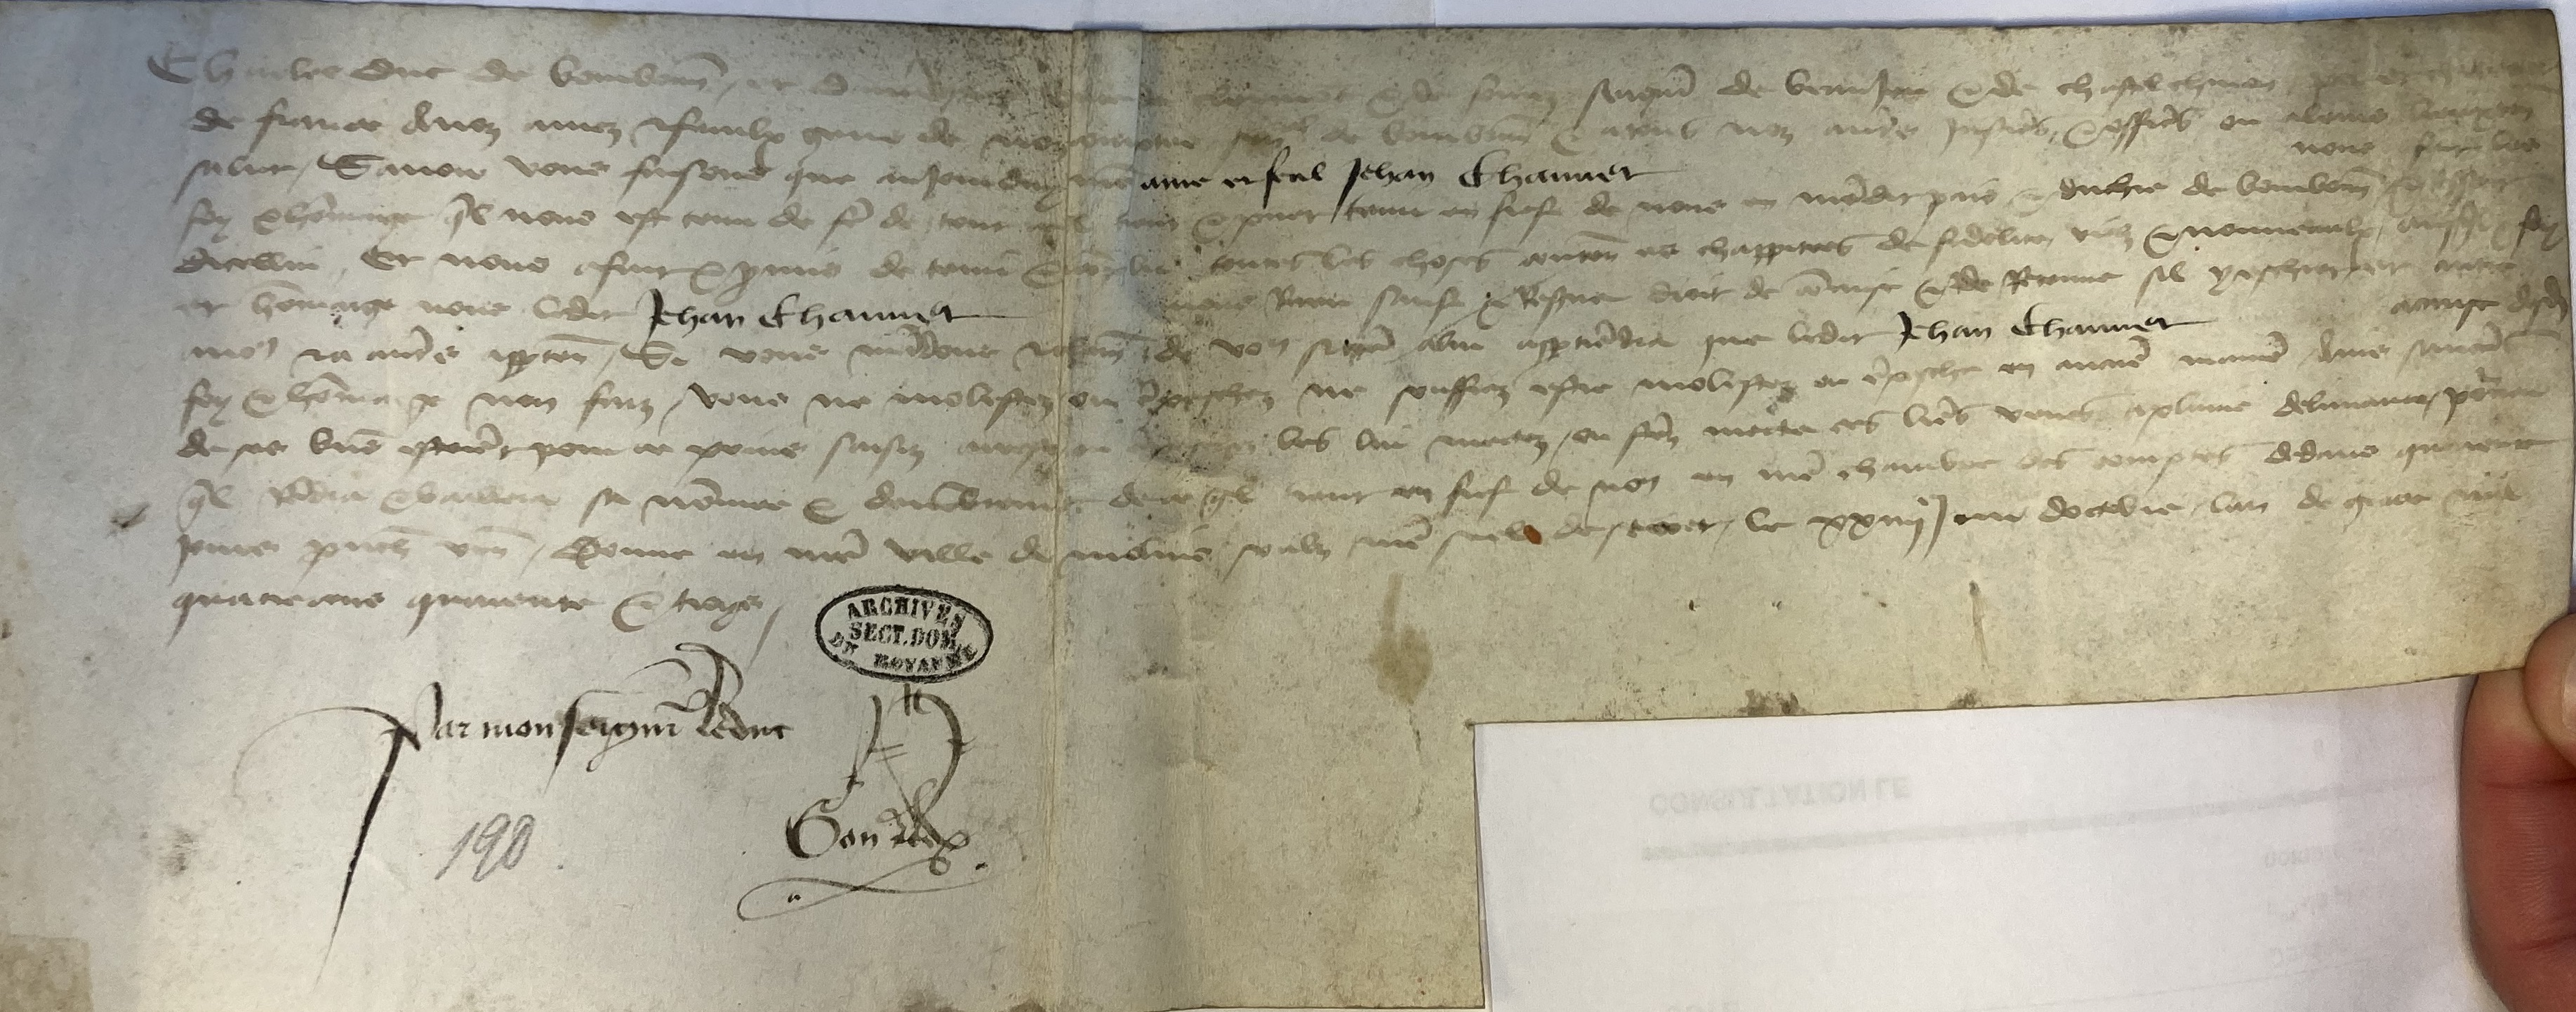
\includegraphics[scale =0.13]{img/IMG-2553.jpg}
\caption*{Acte daté du 24 octobre 1443.}
\label{IMG-2553}
\end{figure}

\begin{figure}[ht]
\centering
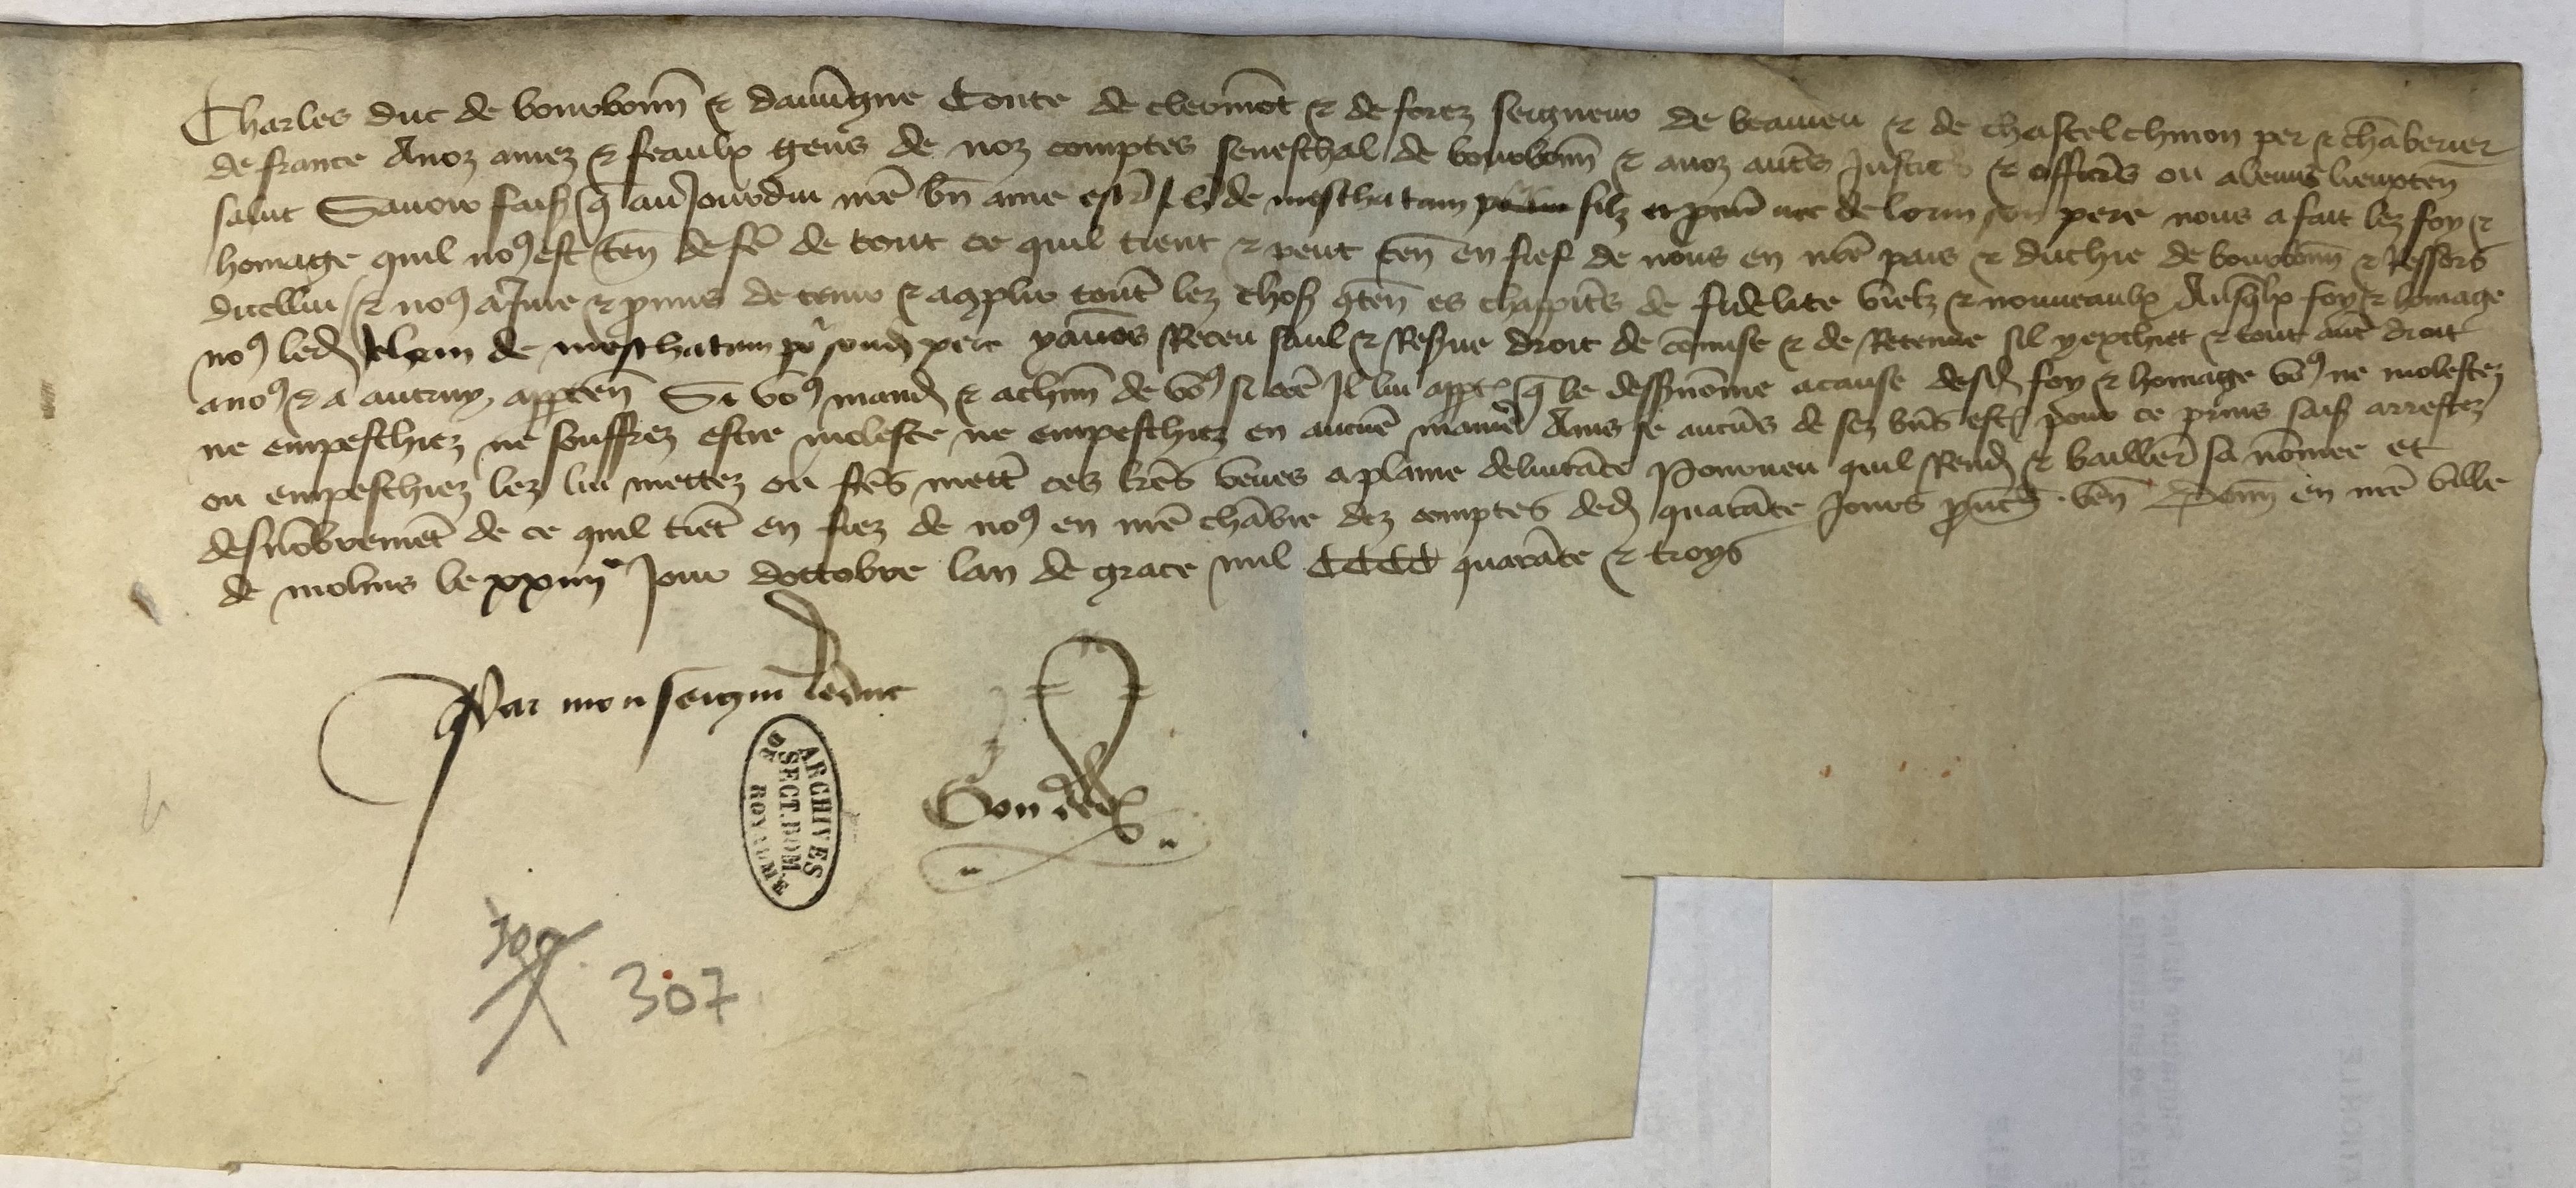
\includegraphics[scale =0.12]{img/IMG-2568.jpg}
\caption*{Acte daté du 24 octobre 1443.}
\label{IMG-2568}
\end{figure}

\begin{figure}[ht]
\centering
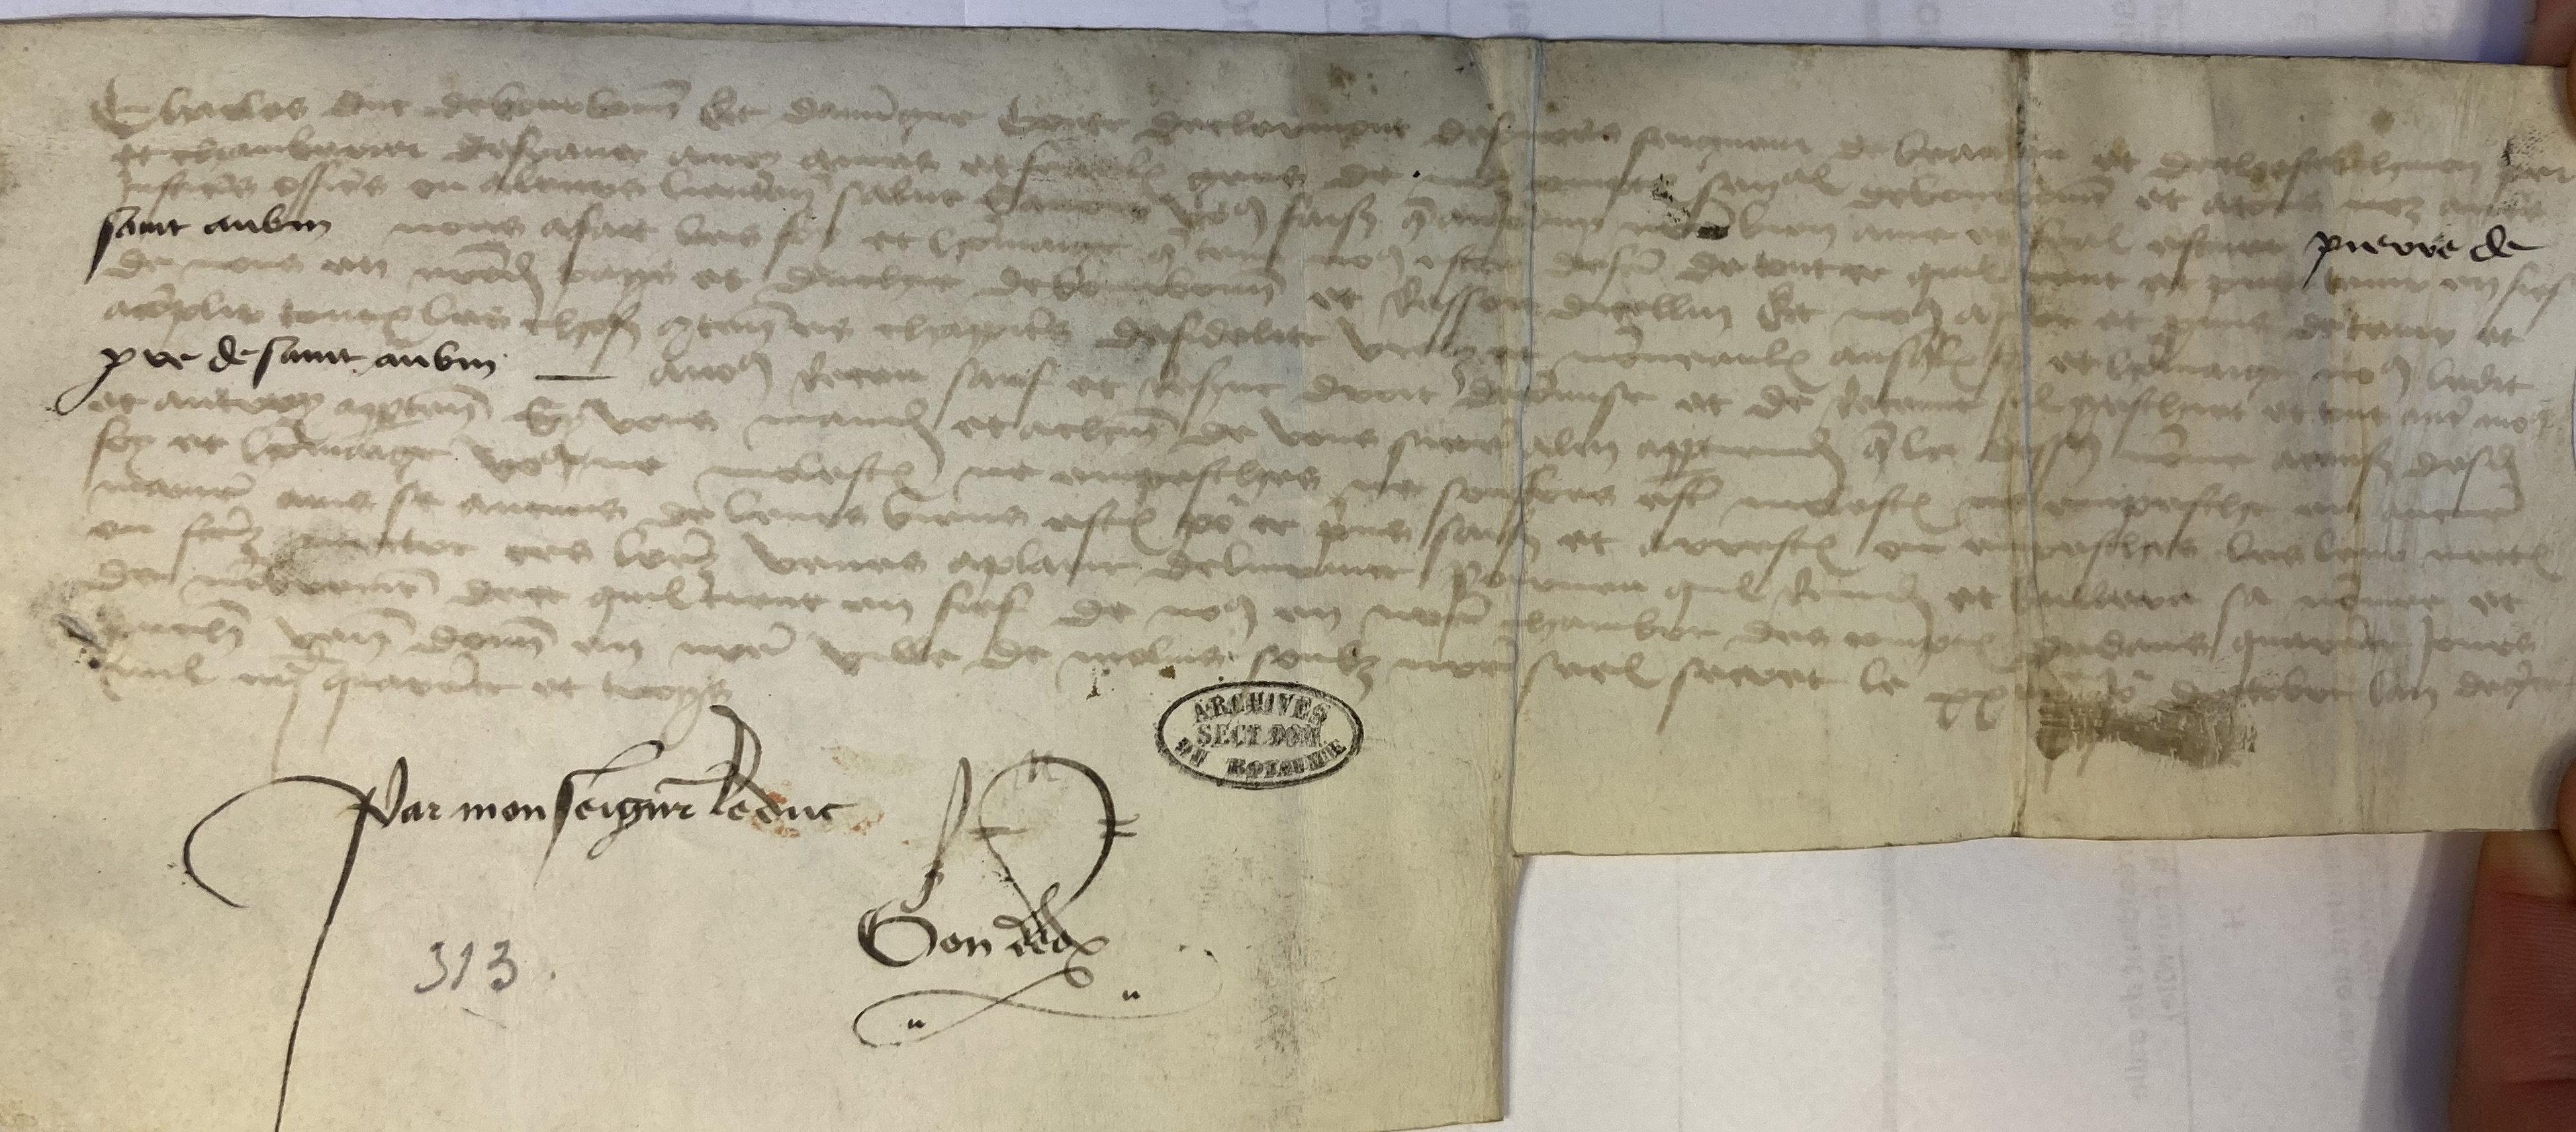
\includegraphics[scale =0.12]{img/IMG-2573.jpg}
\caption*{Acte daté du 24 octobre 1443.}
\label{IMG-2573}
\end{figure}

\begin{figure}[ht]
\centering
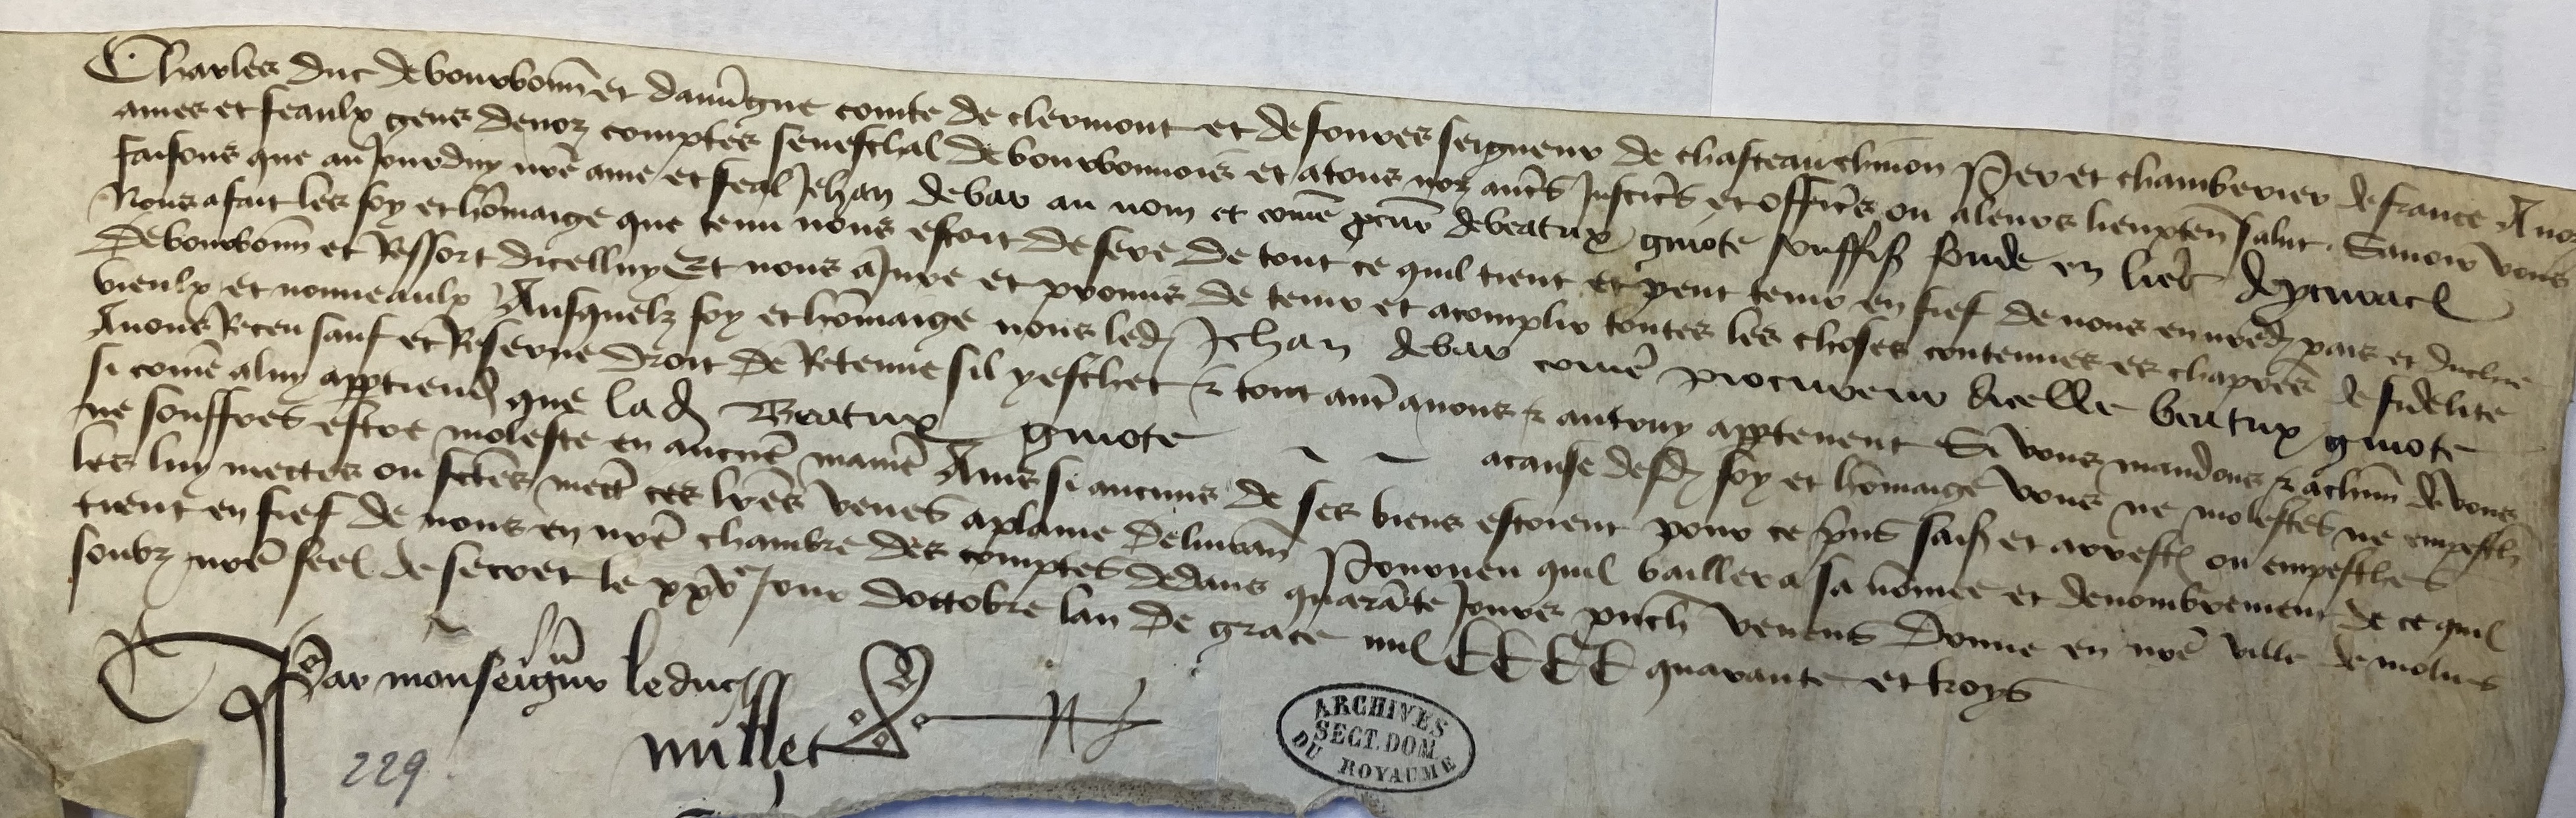
\includegraphics[scale =0.12]{img/IMG-2558.jpg}
\caption*{Acte daté du 25 octobre 1443.}
\label{IMG-2558}
\end{figure}

\begin{figure}[ht]
\centering
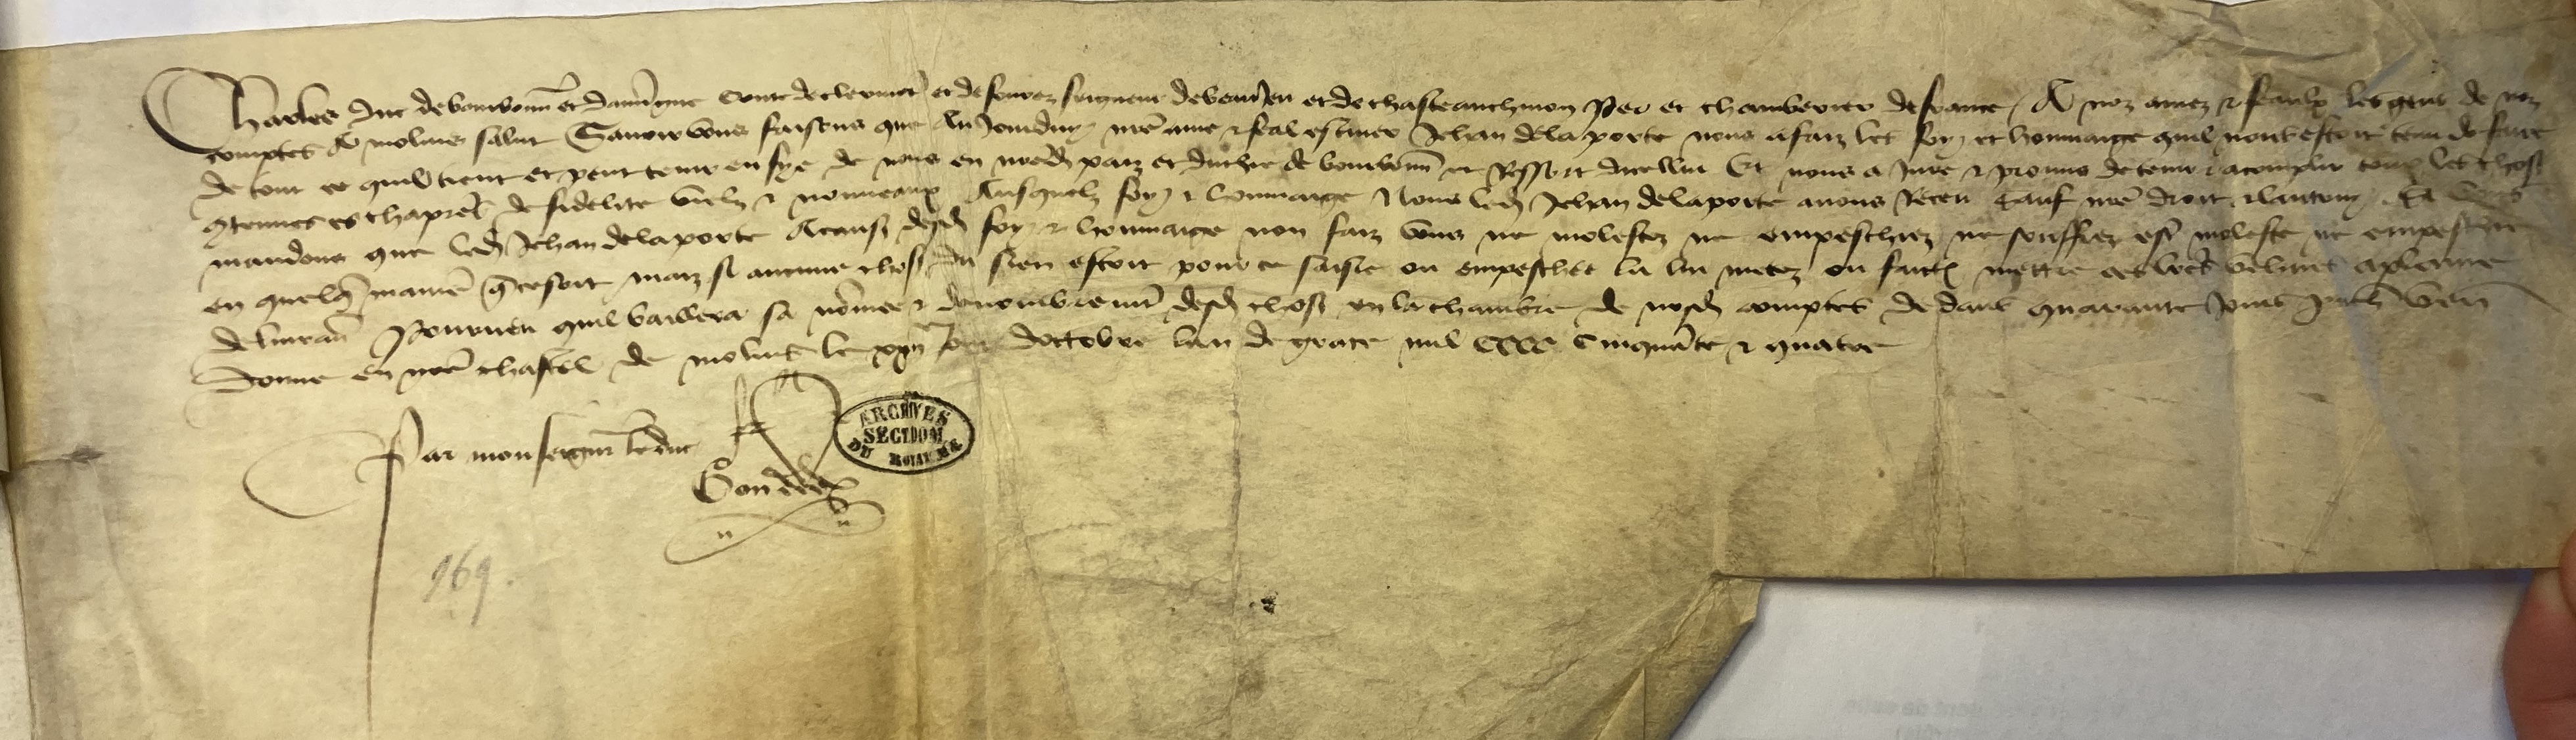
\includegraphics[scale =0.12]{img/IMG-2547.jpg}
\caption*{Acte daté du 22 octobre 1454.}
\label{IMG-2547}
\end{figure}